%%%%%%%%%%%%%%%%%%%%%%%%%%%%%%%%%%%%%%%%%
% Beamer Presentation - LaTeX Template
% Version 2.0 (March 8, 2022)
% Original Template: https://www.LaTeXTemplates.com
% Author: Vel (vel@latextemplates.com)
% License: CC BY-NC-SA 4.0

% Este modelo de apresentação foi 
% criado a partir do modelo de Giovanni Spadaro.
% Disponível em: https://github.com/Giovo17/presentation-template-unict-lm-data
%
% Adaptado por Lucas Amaral Taylor para criar uma versão especial 
% para os alunos de Matemática e Estatística da USP (IME-USP).
% Disponível em: https://github.com/lucasamtaylor01/IME-template
%%%%%%%%%%%%%%%%%%%%%%%%%%%%%%%%%%%%%%%%%

%---------------------------------------------------
% CLASSE DO DOCUMENTO E CONFIGURAÇÕES BÁSICAS
%---------------------------------------------------
\documentclass[
    11pt,               % Tamanho padrão da fonte
    % t,                % Alinhar verticalmente ao topo
    aspectratio=169,   % Definir proporção 16:9
]{beamer}
\graphicspath{{img/}}         % Define o diretório das imagens

%---------------------------------------------------
% PACOTES NECESSÁRIOS
%---------------------------------------------------
\usepackage{
    booktabs,     % Melhora a aparência das linhas em tabelas
    palatino,     % Define Palatino como fonte principal
    subcaption    % Suporte para subfiguras
}
\usepackage[default]{opensans}  % Define Open Sans como fonte secundária
%----------------------------------------------------------------------------------------
%	PACOTES E CONFIGURAÇÕES PARA CÓDIGO
%----------------------------------------------------------------------------------------
% Pacotes necessários para formatação de código
\usepackage[utf8]{inputenc}
\usepackage{listings}
\usepackage{xcolor}

% Cores para syntax highlighting (VSCode Light Theme)
\definecolor{vscBackground}{RGB}{255,255,255}    % Fundo branco
\definecolor{vscKeyword}{RGB}{175,0,219}         % Roxo para palavras-chave
\definecolor{vscString}{RGB}{163,21,21}          % Vermelho para strings
\definecolor{vscComment}{RGB}{0,128,0}           % Verde para comentários
\definecolor{vscFunction}{RGB}{121,94,38}        % Marrom para funções
\definecolor{vscNumber}{RGB}{9,134,88}           % Verde escuro para números
\definecolor{vscOperator}{RGB}{175,0,219}        % Roxo para operadores
\definecolor{vscText}{RGB}{0,0,0}                % Texto preto
\definecolor{vscLineNr}{RGB}{128,128,128}        % Cinza para números de linha

% Configuração geral do listings para UTF-8
\lstset{
    inputencoding=utf8,
    extendedchars=true,
    literate=%
        {á}{{\'a}}1 {é}{{\'e}}1 {í}{{\'i}}1 {ó}{{\'o}}1 {ú}{{\'u}}1
        {Á}{{\'A}}1 {É}{{\'E}}1 {Í}{{\'I}}1 {Ó}{{\'O}}1 {Ú}{{\'U}}1
        {à}{{\`a}}1 {è}{{\`e}}1 {ì}{{\`i}}1 {ò}{{\`o}}1 {ù}{{\`u}}1
        {À}{{\`A}}1 {È}{{\'E}}1 {Ì}{{\`I}}1 {Ò}{{\`O}}1 {Ù}{{\`U}}1
        {ã}{{\~a}}1 {ẽ}{{\~e}}1 {ĩ}{{\~i}}1 {õ}{{\~o}}1 {ũ}{{\~u}}1
        {Ã}{{\~A}}1 {Ẽ}{{\~E}}1 {Ĩ}{{\~I}}1 {Õ}{{\~O}}1 {Ũ}{{\~U}}1
        {â}{{\^a}}1 {ê}{{\^e}}1 {î}{{\^i}}1 {ô}{{\^o}}1 {û}{{\^u}}1
        {Â}{{\^A}}1 {Ê}{{\^E}}1 {Î}{{\^I}}1 {Ô}{{\^O}}1 {Û}{{\^U}}1
        {ç}{{\c c}}1 {Ç}{{\c C}}1
        {º}{{\textordmasculine}}1
        {ª}{{\textordfeminine}}1
}

% Configurações base comum para todas as linguagens
\lstdefinestyle{baseStyle}{
    backgroundcolor=\color{vscBackground},
    basicstyle=\ttfamily\small\color{vscText},
    breakatwhitespace=false,
    breaklines=true,
    captionpos=b,
    keepspaces=true,
    numbers=left,
    numbersep=5pt,
    showspaces=false,
    showstringspaces=false,
    showtabs=false,
    tabsize=4,
    frame=single,
    framerule=0.8pt,
    rulecolor=\color{gray!20},
    numberstyle=\tiny\color{vscLineNr},
    keywordstyle=\color{vscKeyword},
    commentstyle=\color{vscComment}\itshape,
    stringstyle=\color{vscString},
    emphstyle=\color{vscFunction},
    columns=flexible,
    basewidth={0.5em,0.45em},
    inputencoding=utf8,
    extendedchars=true
}

%----------------------------------------------------------------------------------------
% Python
%----------------------------------------------------------------------------------------
\lstdefinestyle{pythonStyle}{
    style=baseStyle,
    language=Python,
    morekeywords={self,None,True,False,import,from,as,def,class,return,yield,
                  for,while,if,else,elif,try,except,finally,with,lambda,
                  async,await,break,continue,global,nonlocal,pass,raise},
    morekeywords=[2]{print,len,range,type,int,str,float,list,dict,set,
                     tuple,max,min,sum,sorted,enumerate,zip,map,filter,
                     any,all,abs,round,pow,divmod},
    keywordstyle=[2]\color{vscFunction},
    sensitive=true
}

\lstnewenvironment{python}[1][]{\lstset{style=pythonStyle, #1}}{}
\newcommand{\pyinline}[1]{\lstinline[style=pythonStyle]!#1!}
\newcommand{\inputpython}[2][]{\lstinputlisting[style=pythonStyle,#1]{#2}}

%----------------------------------------------------------------------------------------
% C Language
%----------------------------------------------------------------------------------------
\lstdefinestyle{cStyle}{
    style=baseStyle,
    language=C,
    morekeywords={include,define,void,int,char,float,double,long,unsigned,
                  struct,union,enum,typedef,const,static,extern,register,
                  auto,volatile,sizeof,return,if,else,for,while,do,switch,
                  case,break,continue,default,goto},
    morekeywords=[2]{printf,scanf,malloc,free,calloc,realloc,fopen,fclose,
                     fprintf,fscanf,strcpy,strlen,strcat},
    keywordstyle=[2]\color{vscFunction},
    sensitive=true
}

\lstnewenvironment{clang}[1][]{\lstset{style=cStyle, #1}}{}
\newcommand{\clinline}[1]{\lstinline[style=cStyle]!#1!}
\newcommand{\inputclang}[2][]{\lstinputlisting[style=cStyle,#1]{#2}}

%----------------------------------------------------------------------------------------
% C++
%----------------------------------------------------------------------------------------
\lstdefinestyle{cppStyle}{
    style=baseStyle,
    language=C++,
    morekeywords={class,private,protected,public,template,typename,namespace,
                  using,new,delete,this,friend,virtual,override,final,explicit,
                  mutable,constexpr,nullptr,noexcept,static_cast,dynamic_cast,
                  const_cast},
    morekeywords=[2]{cout,cin,endl,vector,string,map,set,queue,stack,pair,
                     begin,end,push_back,pop_back,emplace_back,size,empty},
    keywordstyle=[2]\color{vscFunction},
    sensitive=true
}

\lstnewenvironment{cpp}[1][]{\lstset{style=cppStyle, #1}}{}
\newcommand{\cppinline}[1]{\lstinline[style=cppStyle]!#1!}
\newcommand{\inputcpp}[2][]{\lstinputlisting[style=cppStyle,#1]{#2}}

%----------------------------------------------------------------------------------------
% R Language
%----------------------------------------------------------------------------------------
\lstdefinestyle{rStyle}{
    style=baseStyle,
    language=R,
    morekeywords={if,else,repeat,while,function,for,in,next,break,TRUE,FALSE,
                  NULL,Inf,NaN,NA,NA_integer_,NA_real_,NA_complex_,NA_character_},
    morekeywords=[2]{library,require,attach,detach,source,setwd,options,
                     data.frame,read.csv,write.csv,list,matrix,array},
    keywordstyle=[2]\color{vscFunction},
    sensitive=true
}

\lstnewenvironment{rlang}[1][]{\lstset{style=rStyle, #1}}{}
\newcommand{\rlinline}[1]{\lstinline[style=rStyle]!#1!}
\newcommand{\inputrlang}[2][]{\lstinputlisting[style=rStyle,#1]{#2}}

%----------------------------------------------------------------------------------------
% Java
%----------------------------------------------------------------------------------------
\lstdefinestyle{javaStyle}{
    style=baseStyle,
    language=Java,
    morekeywords={abstract,assert,boolean,break,byte,case,catch,char,class,
                  const,continue,default,do,double,else,enum,extends,final,
                  finally,float,for,if,implements,import,instanceof,int,
                  interface,long,native,new,package,private,protected,public,
                  return,short,static,strictfp,super,switch,synchronized,this,
                  throw,throws,transient,try,void,volatile,while},
    morekeywords=[2]{String,System,out,println,printStackTrace,ArrayList,
                     HashMap,Arrays,List,Map,Set,Exception,RuntimeException},
    keywordstyle=[2]\color{vscFunction},
    sensitive=true
}

\lstnewenvironment{java}[1][]{\lstset{style=javaStyle, #1}}{}
\newcommand{\javainline}[1]{\lstinline[style=javaStyle]!#1!}
\newcommand{\inputjava}[2][]{\lstinputlisting[style=javaStyle,#1]{#2}}       % Importa configurações para highlight de código

%---------------------------------------------------
% CONFIGURAÇÃO DO TEMA
%---------------------------------------------------
% Tema Base
\usetheme{Boadilla}                          % Define o tema principal
\useinnertheme{circles}                      % Tema interno com círculos
\useoutertheme{miniframes}                   % Tema externo com miniframes
\setbeamertemplate{navigation symbols}{}     % Remove símbolos de navegação

% Cores Personalizadas
\definecolor{primaryColor}{RGB}{20,45,105}   % Cor primária - azul escuro
\definecolor{secondaryColor}{RGB}{0,100,160} % Cor secundária - azul médio

% Configurações de Cores
\setbeamercolor{structure}{fg=primaryColor}
\setbeamercolor{palette primary}{bg=primaryColor, fg=white}
\setbeamercolor{palette secondary}{bg=secondaryColor, fg=white}
\setbeamercolor{title}{bg=primaryColor, fg=white}

% Cores do Cabeçalho e Rodapé
\setbeamercolor{headline}{bg=secondaryColor, fg=white}
\setbeamercolor{section in head/foot}{bg=primaryColor, fg=white}
\setbeamercolor{subsection in head/foot}{bg=secondaryColor, fg=white}
\setbeamercolor{author in head/foot}{bg=primaryColor, fg=white}
\setbeamercolor{title in head/foot}{bg=secondaryColor, fg=white}
\setbeamercolor{date in head/foot}{bg=primaryColor, fg=white}
\setbeamercolor{page number in head/foot}{bg=primaryColor, fg=white}

\usepackage{multicol}
\usepackage{tikz}

%---------------------------------------------------
% BIBLIOGRAFIA
%---------------------------------------------------
\usepackage[style=alphabetic,backend=biber]{biblatex}
\addbibresource{bibliografia.bib}

%---------------------------------------------------
% INFORMAÇÕES DA APRESENTAÇÃO
%---------------------------------------------------
\title[Lorenz 80]{Um breve estudo do Modelo Lorenz 80}
\author[TAYLOR, Lucas A.]{Lucas Amaral Taylor}            
\institute[IME-USP]{Instituto de Matemática e Estatística \\ (IME-USP)}
\date{Fevereiro de 2025}

%---------------------------------------------------
% INÍCIO DO DOCUMENTO
%---------------------------------------------------
\begin{document}

% Slide de título com logo
\begin{frame}
    \begin{figure}
        
\includegraphics[width=0.4\linewidth]{img/logo_IME.png}
    \end{figure}
    \titlepage
\end{frame}

% Sumário
\begin{frame}
    \frametitle{Estrutura da apresentação}
    \tableofcontents
\end{frame}

% Inclusão das seções
\section{Introdução} % Seções são adicionadas para organizar sua apresentação em blocos discretos, todas as seções e subseções são automaticamente exibidas no índice como uma visão geral da apresentação, mas NÃO são exibidas como slides separados.

%----------------------------------------------------------------------------------------

\begin{frame}
	\frametitle{Objetivos da apresentação}
    \begin{enumerate}
        \item Apresentação geral do artigo de Lorenz
        \item Relacionar os assuntos apresentados em aula com os temas abordados no artigo. 
        \item 
    \end{enumerate}

\end{frame}

%------------------------------------------------------------------------------------

\section{Construção dos modelos} 

% ----------------------------

\begin{frame}{\textit{PE Model}: Características do fluido}
	\begin{itemize}
		\item \textbf{Homogêneo.} A densidade do fluido é uniforme em todo volume;
		\item \textbf{Incompressível.} O volume não muda quando submetido à pressão ($\nabla \cdot V = 0$)
	\end{itemize}
\end{frame}

% ----------------------------

\begin{frame}{\textit{PE Model}: O modelo de água rasa}
		
	Fazendo as devidas alterações notacionais em \cite{salmon1998}, temos:
	\begin{align}
		\frac{\partial V}{\partial t} + (V \cdot \nabla)V + f \mathbf{k} \times V & = -g \nabla z \label{eq:agua-rasa-1} \\
		\frac{\partial z}{\partial t} + \nabla \cdot (z V)                        & = 0 \label{eq:agua-rasa-2}           
	\end{align}
		
	\begin{small}
		Onde:
		\begin{multicols}{2}
			\begin{itemize}
				\item $t$: tempo;
				\item $\mathbf{r}$: vetor de posição inicial;
				\item $V(t,r)$: Velocidade horizontal;
				\item $z(t,r)$: altura da superfície;
				\item $f$: parâmetro de Coriolis;
				\item $g$: aceleração da gravidade;
				\item $\mathbf{k}$: vetor da vertical.
			\end{itemize}
		\end{multicols}
	\end{small}
\end{frame}

% ----------------------------

\begin{frame}{\textit{PE Model}: Modelo de água rasa}


\begin{center}
    \begin{tikzpicture}
    \draw[blue, thick] (0,4) to[out=0,in=180] (1,4.2) 
                            to[out=0,in=180] (2,3.8)
                            to[out=0,in=180] (3,4.2)
                            to[out=0,in=180] (4,3.8)
                            to[out=0,in=180] (5,4.2)
                            to[out=0,in=180] (6,3.8);
    \node[blue, right] at (6,3.8) {Superfície};
    
    % Anotação do desvio z - agora apontando para cima a partir do vale
    \draw[blue] (2,3.8) -- (2,4.3);  % Linha vertical para cima a partir do vale
    \node[blue] at (2,4.6) {$z$: desvio da superfície do fluido};
    
    % Velocidade V(t,r)
    \node[red] at (2,3) {$V(t,r) \rightarrow$};
    
    % Profundidade média H
    \draw[black] (4,3.8) -- (4,1.8);
    \node[right] at (4,3) {$H$: profundidade média};
    
    % Topologia do fundo (curva inferior)
    \draw[red, thick] (0,2) to[out=10,in=170] (2,2.3) to[out=350,in=170] (4,1.8) to[out=350,in=170] (6,2);
    
    % Variação h
    \draw[red] (2,2.3) -- (2,1.8);
    \node[red] at (3,1.3) {$h$: variação da topologia do fundo};

\end{tikzpicture}
\end{center}

\end{frame}

% ----------------------------

\begin{frame}{\textit{PE Model}: O modelo de água rasa modificado}
	\begin{small}
		No artigo, nos é apresentado as seguintes equações:
		\begin{align}
			\frac{\partial V}{\partial t} & = - ( V \cdot \nabla)V - f \mathbf{k} \times V - g \nabla z + \nu \nabla^2\mathbf{V} \label{eq:agua-rasa-modificada-1}     \\
			\frac{\partial z}{\partial t} & = - (V \cdot \nabla)(z - h) - (H + z - H)\nabla \cdot \mathbf{V} + \kappa \nabla^2 z + F \label{eq:agua-rasa-modificada-2} 
		\end{align}
	\end{small}
	\begin{scriptsize}
		Onde:
		\begin{multicols}{2}
			\begin{itemize}
				\item $t$: tempo
				\item $\mathbf{r}$: vetor de posição inicial;
				\item $H$: profundidade média do fluido;
				\item $h(r)$: variação da superfície topológica;
				\item $V(t,r)$: Velocidade horizontal;
				\item $z(t,r)$: altura da superfície;
				\item $f$: parâmetro de Coriolis;
				\item $g$: aceleração da gravidade;
				\item $F$: forças externas;
				\item $\kappa$: coeficiente de difusão viscosa;
				\item $\nu$: coeficiente de difusão térmica;
				\item $\mathbf{k}$: vetor da vertical.
			\end{itemize}
		\end{multicols}
	\end{scriptsize}
\end{frame}

% ----------------------------

\begin{frame}{\textit{PE Model}: Sobre os processos de difusão}
	Nas equações \eqref{eq:agua-rasa-modificada-1} e \eqref{eq:agua-rasa-modificada-2}, temos dois processos de difusão:
	\begin{enumerate}
		\item \textbf{Difusão viscosa:} transferência do momento entre partes do fluido devido à viscosidade \textit{(exemplo: mel)};
		\item \textbf{Difusão térmica:} Transferência de calor por condução entre regiões com diferentes temperaturas.
	\end{enumerate}
		
	\begin{small}
	    \textit{Observação: Ambos os processos tendem a uniformizar suas respectivas propriedades.}
	\end{small}
\end{frame}

% ----------------------------
\begin{frame}{\textit{PE Model}: Algumas observações das equações \eqref{eq:agua-rasa-modificada-1} e \eqref{eq:agua-rasa-modificada-2}}
	\begin{enumerate}
		\item A média horizontal de $h$ e $z$ é zero;
		\item $V(t,r)$ e $z(t,r)$ são amortecidas pelo processo de difusão de pequenas escala, este fato auxilia na simulação de fenômenos atmosféricos;
		\item O ``efeito $\beta$'', efeito que indica como o movimento do fluido é afetado pelas alterações espaciais do parâmetro Coriolis, é suprimido da equação \eqref{eq:agua-rasa-modificada-2}, através da escolha da topografia. Tal decisão baseia-se no artigo \cite{von_arx1952} que prova o fato teoricamente e laboratorialmente. 
	\end{enumerate}
\end{frame}



% ----------------------------
\begin{frame}{\textit{PE Model}: A formação de novas equações}
	A partir da \textit{Decomposição de Helmholtz}, decomposição que divide a \textit{parte rotacional} e a parte \textit{divergente}, aplicada a equação \eqref{eq:agua-rasa-modificada-2}, temos:
	
	\begin{equation}
		V = \nabla\chi + \mathbf{k} \times \nabla \psi \label{eq:decomposicao-helmholtz}
	\end{equation}
	
	Onde:
	\begin{itemize}
		\item $\chi$: potencial de velocidade (\textit{parte divergente})
		\item $\psi$: função corrente (\textit{parte rotacional})
		\item $\mathbf{k}$: vetor unitário vertical
	\end{itemize}
\end{frame}

% ----------------------------

\begin{frame}{\textit{PE Model}: A formação de novas equações}
   A partir da equação \eqref{eq:decomposicao-helmholtz} e \eqref{eq:agua-rasa-modificada-1}, obtemos as duas seguintes equações:
   \begin{small}
       \begin{align}
           \frac{\partial \nabla^2 \chi}{\partial t} &= -\frac{1}{2}\nabla^2(\nabla \chi \cdot \nabla \chi) - \nabla \chi \cdot \nabla(\nabla^2\psi) \times \mathbf{k} + \nabla^2(\nabla \chi \cdot \nabla \psi \times \mathbf{k}) \nonumber \\
           &\quad + \nabla \cdot (\nabla^2\psi\nabla\psi) - \frac{1}{2}\nabla^2(\nabla \psi \cdot \nabla \psi) + \nu\nabla^4\chi + f\nabla^2\psi - g\nabla^2z \label{eq:equacao-basica-1} \\
           \frac{\partial \nabla^2 \psi}{\partial t} &= -\nabla \cdot (\nabla^2\psi\nabla \chi) - \nabla \psi \cdot \nabla(\nabla^2\psi) \times \mathbf{k} - f\nabla^2\chi + \nu\nabla^4\psi\label{eq:equacao-basica-2}
       \end{align}
   \end{small}

   Onde:
   \begin{itemize}
       \item $\frac{\partial \nabla^2 \chi}{\partial t}$: expressa a vorticidade;
       \item $\frac{\partial \nabla^2 \psi}{\partial t}$: expressa o divergente
   \end{itemize}
\end{frame}

% ----------------------------

\begin{frame}{\textit{PE Model}: A formação de novas equações}
   Realizando o mesmo processo, a partir das equações \eqref{eq:agua-rasa-modificada-2} e \eqref{eq:decomposicao-helmholtz}, obtemos a seguinte equação:
    \begin{equation}
        \frac{\partial z}{\partial t} = -\nabla \cdot (z - h)\nabla \chi - \nabla \psi \cdot \nabla(z - h) \times \mathbf{k} - H\nabla^2\chi + \kappa\nabla^2z + F \label{eq:equacao-basica-3}
    \end{equation}

    As equações \eqref{eq:equacao-basica-1}, \eqref{eq:equacao-basica-2} e \eqref{eq:equacao-basica-3} serão as equações básicas para a construção do modelo de baixa ordem
\end{frame}

% ----------------------------

\begin{frame}{\textit{PE Model:} Objetivos do Processo de simplificação}

\begin{enumerate}
    \item Converter as equações \eqref{eq:equacao-basica-1}, \eqref{eq:equacao-basica-2} e \eqref{eq:equacao-basica-3} para um modelo de baixa ordem. 
    \item Transformaremos um modelo formado originalmente por equações primitivas atmosféricas em um sistema de nove variáveis.
\end{enumerate}
    
\end{frame}

% ----------------------------

\begin{frame}{\textit{PE Model}: Processo de simplificação}

Primeiro, introduziremos três vetores adimensionais, que respeitam a seguinte condição:
\begin{equation}
    \alpha_1 + \alpha_2 + \alpha_3 = 0
\end{equation}

Junto a permutação abaixo:
\begin{equation}
    (i, j, k) = (1,2,3), (2,3,1), (3,1,2) \label{eq:permutacao}
\end{equation}

Definiremos as variáveis $a_i, b_i$ e $c_i$
\end{frame}

% ----------------------------

\begin{frame}{\textit{PE Model}: Processo de simplificação}

As variavéis $a_i, b_i$ e $c_i$ são definidas da seguinte forma:
\begin{align*}
    a_i &= \alpha_1 \cdot \alpha_j\\
    b_i &= \alpha_j \cdot \alpha_i\\
    c_i &= \alpha_j \times \alpha_k \cdot \mathbf{k}
\end{align*}

\textit{Observação: Apesar dessa relação ser  válida, Lorenz apresenta outra (esta foi usado na aplicação computacional)}:
\begin{align*}
    b_i &= \frac{1}{2}\left(a_i - a_j - a_k\right)\\
    c_i &= c
\end{align*}
\end{frame}

% ----------------------------

\begin{frame}{\textit{PE Model}: Processo de simplificação}
    Por fim, definimos um comprimento $L$ e criamos três funções ortogonais:
    \begin{equation*}
        \phi_i = \cos\left(\alpha_i \cdot \frac{r}{L}\right)
    \end{equation*}

    A partir delas, temos:
    \small
    \begin{align*}
        L^2\nabla^2\phi_i &= -a_i\phi_i \\
        L^2\nabla\phi_i \cdot \nabla\phi_k &= -\frac{1}{2}b_{ik}\phi_i + \cdots \\
        L^2\nabla \cdot (\phi_j\nabla\phi_k) &= \frac{1}{2}b_{jk}\phi_i + \cdots \\
        L^2\phi_j \cdot \nabla\phi_k \times \mathbf{k} &= -\frac{1}{2}c_{jk}\phi_i + \cdots
    \end{align*}
\end{frame}

% ----------------------------

\begin{frame}{\textit{PE Model}: Processo de simplificação}
    A partir delas, podemos introduzir as variáveis adimensionais normalizadas:
    \begin{align}
        t &= f^{-1}\tau \label{eq:variaveis-adimensionais-inicio}\\
        \chi &= 2L^2f^2 \sum x_i\phi_i \\
        \psi &= 2L^2f^2 \sum y_i\phi_i \\
        z &= 2L^2f^2g^{-1} \sum z_i\phi_i \\
        h &= 2L^2f^2g^{-1} \sum h_i\phi_i \\
        F &= 2L^2f^2g^{-1} \sum F_i\phi_i \label{eq:variaveis-adimensionais-fim}
    \end{align}
\end{frame}


% ----------------------------

\begin{frame}{\textit{PE Model}: Processo de simplificação}
    Em seguida, aplicamos as variáveis definidas em \eqref{eq:variaveis-adimensionais-inicio}-\eqref{eq:variaveis-adimensionais-fim}, nas equações \eqref{eq:equacao-basica-1}, \eqref{eq:equacao-basica-2} e \eqref{eq:equacao-basica-3}, obtemos as seguintes equações:

    \begin{small}
        \begin{align}
       a_i\frac{dx_i}{d\tau} &= a_ib_1x_ix_k - c(a_i - a_k)x_iy_k  c(a_i - a_j)y_ix_k\nonumber\\
       &-2c^2y_iy_k - \nu_0a_i^2x_i + a_iy_i - a_iz_i \label{eq:equacao-principal-1}\\
       a_i\frac{dy_i}{d\tau} &= -a_ib_kx_iy_k - a_ib_iy_ix_k + c(a_k - a_i)y_iy_k - a_ix_i - \nu_0a_i^2y_i \label{eq:equacao-principal-2}\\
       \frac{dz_i}{d\tau} &= -b_kx_i(z_k - h_k) - b_i(z_i - h_i)x_k + cy_i(z_k - h_k) \nonumber\\
       &- c(z_i - h_i)y_k + g_0a_ix_i - \kappa_0a_iz_i + F_i \label{eq:equacao-principal-3}
    \end{align}
    \end{small}
\end{frame}


% ----------------------------

\begin{frame}{\textit{PE Model:} Breves observações}

\begin{itemize}
    \item As variáveis com o índice 1 representam campos de velocidade e altura zonalmente uniformes

    \item As variáveis com o índice 2 ou 3 representam ondas ou redemoinhos de grande escala sobrepostos.

    \item Este modelo será usado em simulações e levará em consideração a permutação \eqref{eq:permutacao}
\end{itemize}
\end{frame}


% ----------------------------

\begin{frame}{\textit{PE Model:} Mais um processo de simplificação}

Primeiro, definiremos $U$ e $V$:
\begin{align}
   U_i &= -b_ix_i + cy_i \\
   V_i &= -b_kx_i - cy_i
\end{align}

Em seguida, $X_i$ e $Y_i$:
\begin{align}
    X_i &= -a_ix_i \\
    Y_i &= -a_iy_i
\end{align}

\end{frame}

% ----------------------------

\begin{frame}{\textit{PE Model:} Mais um processo de simplificação}

Aplicando $U, V, X_i$ e $Y_i$ em \eqref{eq:equacao-principal-1}, \eqref{eq:equacao-principal-2} e \eqref{eq:equacao-principal-3}, obtemos:

\begin{align}
    \frac{dX_i}{d\tau} &= U_iU_k + V_jV_k - \nu_0a_iX_i + Y_i + a_iz_i \label{eq:equacao-principal-simplificada-1}\\
    \frac{dY_i}{d\tau} &= U_iY_k + Y_jV_k - X_i - \nu_0a_iY_i \label{eq:equacao-principal-simplificada-2}\\
    \frac{dz_i}{d\tau} &= U_i(z_k - h_k) + (z_j - h_j)V_k - g_0X_i - \kappa_0a_iz_i + F_i \label{eq:equacao-principal-simplificada-3}
\end{align}

Este modelo também segue as permutações de \eqref{eq:permutacao} e também será usado em simulações numéricas.

\end{frame}

% ----------------------------

\begin{frame}{\textit{QG Model}: Construção do modelo}

Da equação \eqref{eq:equacao-principal-1}:
\begin{itemize}
    \item Elimina-se todos os termos que contém $x$, inclusive aqueles que tem derivada em relação ao tempo
\end{itemize}

Das equações \eqref{eq:equacao-principal-2} e \eqref{eq:equacao-principal-3}:
\begin{itemize}
    \item Elimina-se todos os termos não lineares ou topográficos 
    \item Elimina-se todos os termos com $x$ e $z$
\end{itemize}

\end{frame}

% ----------------------------

\begin{frame}{\textit{QG Model}: Construção do modelo}
A partir deste processo obtem-se:
\begin{align}
    (a_ig_0 + 1)\frac{dy_i}{d\tau} &= g_0c(a_k - a_j)y_jy_k - a_i(a_ig_0v_0 + \kappa_0)y_i\nonumber \\ 
    &\quad - ch_ky_j + ch_jy_k + F_i \label{eq:qg-model}
\end{align}

	\begin{small}
		Onde:
			\begin{itemize}
                \item $(a_ig_0 + 1)\frac{dy_i}{d \tau}$: termo de evolução temporal
                \item $g_oc(a_k - a_j)y_jy_k$: Advecção da vorticidade planetária
                \item $-a_i(a_ig_0v_0 + \kappa_0)y_i$: dissipação
			    \item $- ch_ky_j + ch_jy_k$: efeitos topográficos
                \item $F_i$: forçamento
            \end{itemize}
	\end{small}
\end{frame}


\section{Simulações} % Seções são adicionadas para organizar sua apresentação em blocos discretos, todas as seções e subseções são automaticamente exibidas no índice como uma visão geral da apresentação, mas NÃO são exibidas como slides separados.

%----------------------------------------------------------------------------------------
\begin{frame}[fragile]
    \frametitle{Python}
    
    \begin{python}
def calcular_dobro(x):
    """Retorna o dobro do número"""
    return 2 * x

# Testando a função
numero = 5
resultado = calcular_dobro(numero)
print(f"O dobro de {numero} é {resultado}")
    \end{python}
\end{frame}


    \section{Simulações}

%---------------------------------------------------

\begin{frame}{\textit{Modelo PE}: Processo de simulação}
	
	Dada a seleção do modelo, o seguinte processo é realizado:
	
	\begin{enumerate}
		\item Seleção de constantes e condições iniciais
		\item Método de discretização (RK4)
		\item Plotagem
	\end{enumerate}
\end{frame}


%---------------------------------------------------
\begin{frame}[fragile]
	
	\frametitle{\textit{Modelo PE}: Seleção de constantes}
	    
	\begin{python}
vetor_a = [1, 1, 3]
vetor_b = [
0.5 * (vetor_a[0] - vetor_a[1] - vetor_a[2]),
0.5 * (vetor_a[1] - vetor_a[2] - vetor_a[0]),
0.5 * (vetor_a[2] - vetor_a[0] - vetor_a[1]),
]
c = math.sqrt(3/4)
		
f_inv = 10800
vetor_h = [-1, 0, 0]
vetor_f = [0.1, 0, 0]
g_0 = 8
kappa_0 = 1 / 48
nu_0 = kappa_0
	\end{python}
\end{frame}

%---------------------------------------------------

\begin{frame}{\textit{Método de discretização RK4}: Características gerais}

Um método é de Runge-Kutta explícito de ordem $4$ se, e só se, satisfaz três propriedades:
\begin{enumerate}
    \item Método de passo único explícito;
    \item Apresenta boa estabilidade para equações diferenciais ordinárias (EDOs).
    \item Possui erro global da ordem de $\mathcal{O}(h^4)$, garantindo alta precisão com um custo computacional moderado. 
\end{enumerate}

\end{frame}

%---------------------------------------------------

\begin{frame}{\textit{Método de discretização RK4}: Formulação}

Tomando como referência \cite{roma2023}, podemos expressar o método RK44 da seguinte maneira:
\begin{equation*}
    \Phi(t,y,h) = \frac{1}{6} \left( \kappa_1 + 2\kappa_2 + 2\kappa_3 + \kappa_4 \right) \quad \text{com} \quad
    \begin{cases}
        \kappa_1 = f(t,y) \\
        \kappa_2 = f \left( t + h/2, y + (h/2) \kappa_1 \right) \\
        \kappa_3 = f \left( t + h/2, y + (h/2) \kappa_2 \right) \\
        \kappa_4 = f \left( t + h, y + h\kappa_3 \right)
    \end{cases}
    \end{equation*}
\end{frame}

%---------------------------------------------------
\begin{frame}[fragile]
	
	\frametitle{\textit{Modelo PE}: Condições iniciais - padrão}
	Primeira condição inicial, é a dada por padrão e tem o intuito de reproduzir a figura 1 do artigo.    
	\begin{python}
# Condições iniciais
x0 = [0.1, 0, 0]
y0 = [0.1, 0, 0]
z0 = [0.1, 0, 0]
	\end{python}
\end{frame}

%---------------------------------------------------

\begin{frame}{\textit{Modelo PE}: Resultados condição inicial padrão}
	\begin{figure}
		\centering
		\begin{subfigure}[b]{0.45\textwidth}
			\centering
			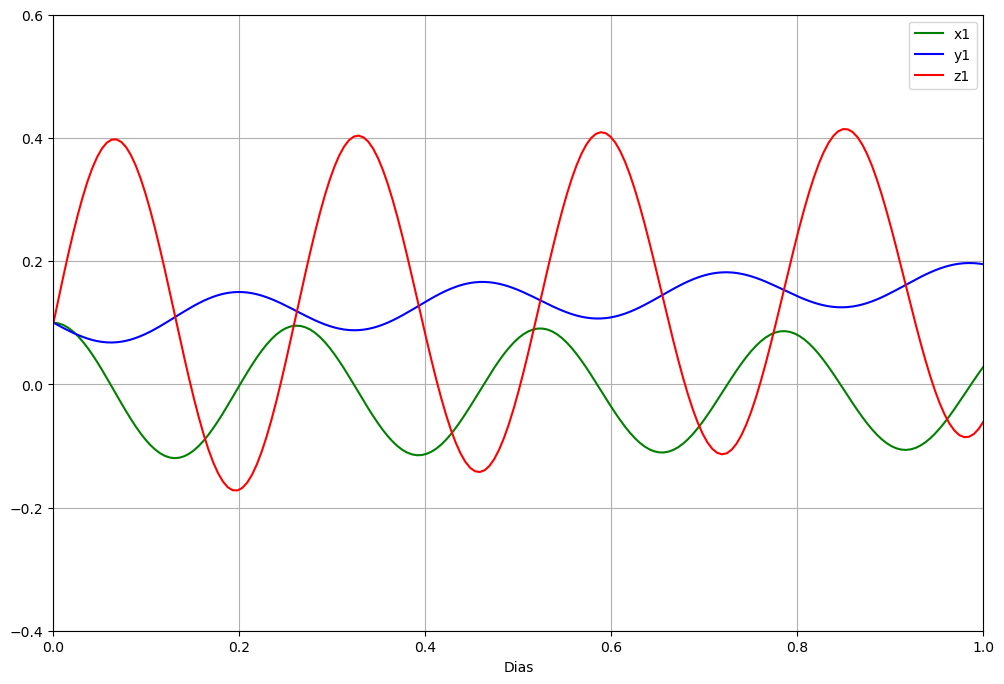
\includegraphics[width=\textwidth]{img/p01d01.png}
			\caption{Condição padrão - 01 dia\\(reprodução)}
			\label{fig:p01d01}
		\end{subfigure}
		\hfill
		\begin{subfigure}[b]{0.45\textwidth}
			\centering
			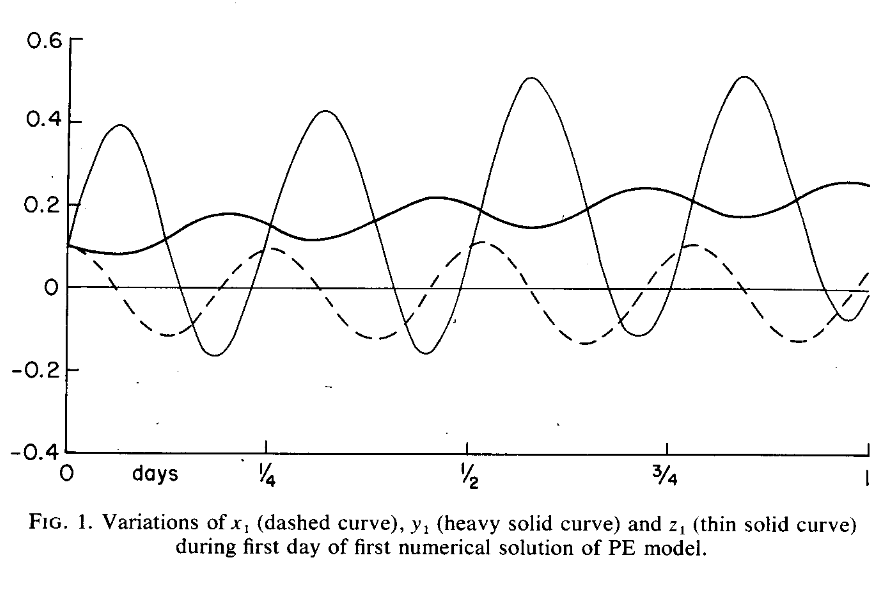
\includegraphics[width=\textwidth]{img/p01d01rel.png}
			\caption{Condição padrão - 01 dia\\(artigo)}
			\label{fig:p01d01rel}
		\end{subfigure}
	\end{figure}
\end{frame}

%---------------------------------------------------

\begin{frame}{\textit{Modelo PE}: Resultados condição inicial padrão}
	\begin{figure}
		\centering
		\begin{subfigure}[b]{0.45\textwidth}
			\centering
			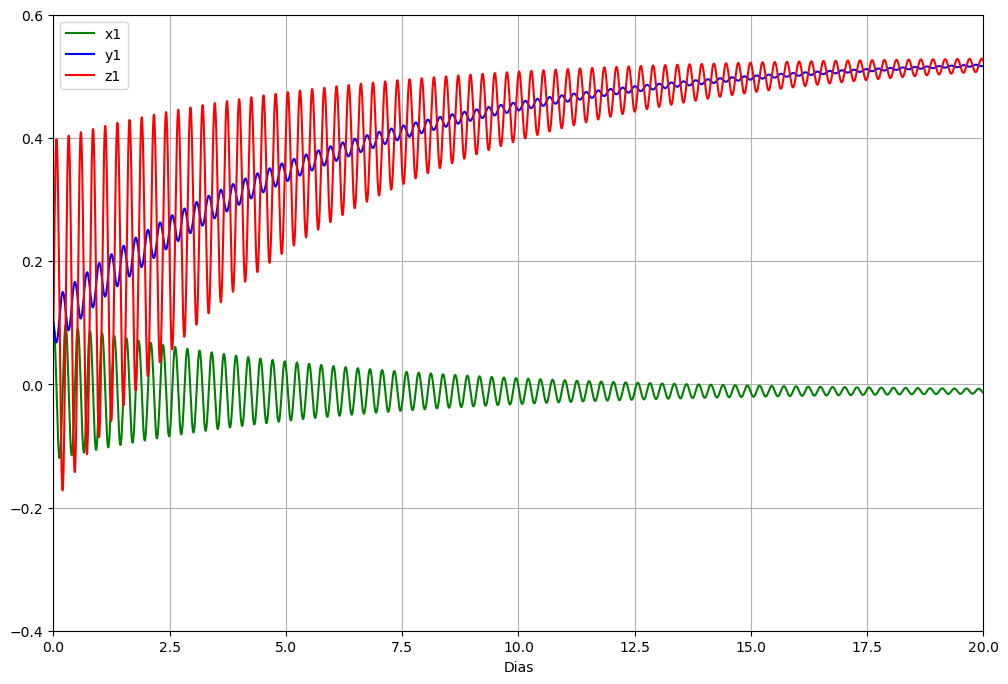
\includegraphics[width=\textwidth]{img/p01d20.png}
			\caption{Condição padrão - 20 dias}
			\label{fig:p01d20}
		\end{subfigure}
		\hfill
		\begin{subfigure}[b]{0.45\textwidth}
			\centering
			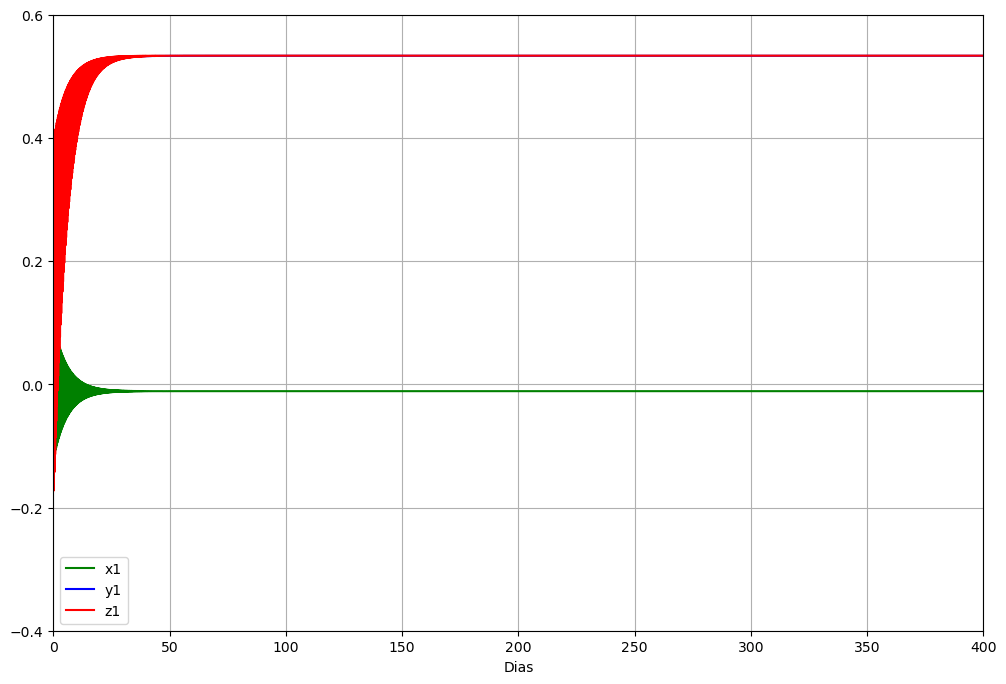
\includegraphics[width=\textwidth]{img/p01d400.png}
			\caption{Condição padrão - 400 dias}
			\label{fig:p01d400}
		\end{subfigure}
	\end{figure}
\end{frame}


%---------------------------------------------------
\begin{frame}{Condições de Hadley}

    A circulação de Hadley é um padrão de circulação atmosférica nos trópicos, onde o ar quente sobe próximo ao equador e desce em latitudes mais altas, formando um ciclo convectivo.
    \begin{itemize}
        \item Em 1735, Hadley incorporou o efeito da rotação da Terra, mostrando que a velocidade do ar varia com a latitude, influenciando a direção predominante dos ventos nos trópicos.
        
        \item Baseia-se na conservação do momento angular, garantindo o equilíbrio do movimento atmosférico e evitando mudanças na rotação da Terra.
        
        \item Responsável pelos ventos predominantes nos trópicos e pela redistribuição de calor na atmosfera, influenciando padrões climáticos globais.
    \end{itemize}
\end{frame}

%---------------------------------------------------

\begin{frame}{\textit{Modelo PE}: Condições iniciais - Hadley 01}
A partir do artigo \cite{gent1982}, temos que os valores dos vetores para as condições de Hadley são definidas como:
	\begin{align*}
        x_1 &= - \nu_0 a_1 y_1, \\
        y_1 &= \frac{F_1}{a_1} v_0 \left( 1 + a_1 g_0 + \nu_0^2 a_1^2 \right), \\
        z_1 &= \left( 1 + \nu_0^2 a_1^2 \right) y_1\\
        x_2 &= y_2 = z_2 = x_3 = y_3 = z_3 = 0
\end{align*}

\end{frame}


%---------------------------------------------------
\begin{frame}[fragile]
	
	\frametitle{\textit{Modelo PE}: Condições iniciais - Hadley 01}
	Adaptando para o código, temos:
	\begin{python}
# Condições iniciais
y1 = (vetor_f[1]
/ vetor_a[1] * nu_0 * (1 + vetor_a[1] * g_0 + nu_0**2 * vetor_a[1] ** 2))
z1 = (1 + nu_0**2 * vetor_a[1] ** 2) * y1
x1 = -nu_0 * vetor_a[1] * y1
		
x_hadley01_inicial = [x1, 0, 0]
y_hadley01_inicial = [y1, -(10 ** (-5)), 0]
z_hadley01_inicial = [z1, 10 ** (-5), 0]
	\end{python}
\end{frame}

%---------------------------------------------------

\begin{frame}{\textit{Modelo PE}: Resultados para condição de Hadley 01}
	\begin{figure}
		\centering
		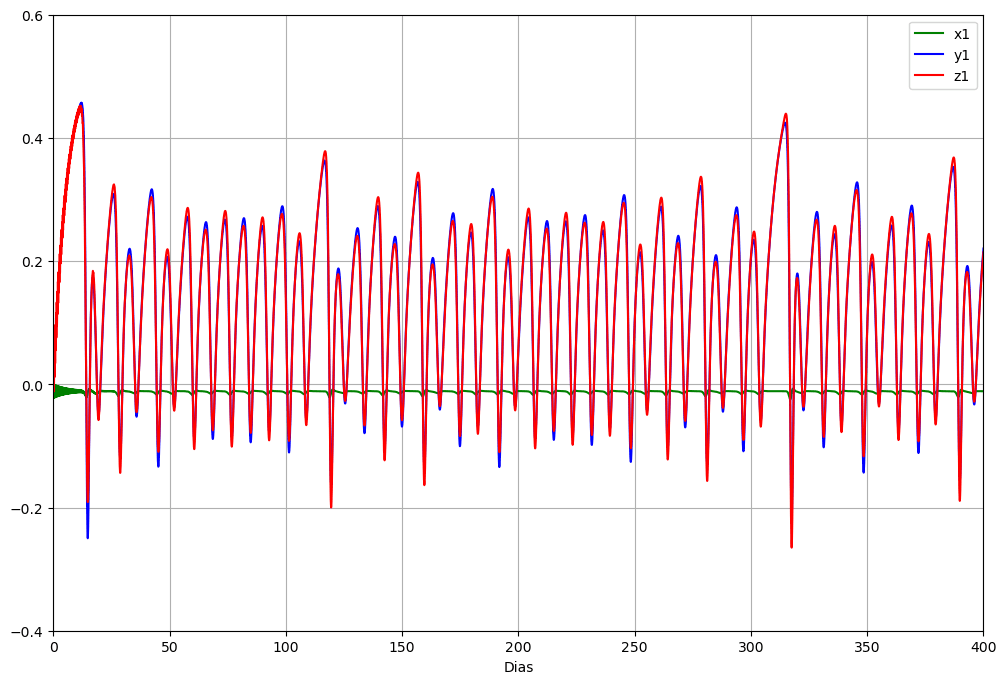
\includegraphics[width=0.5\textwidth]{img/p02d260.png}
		\caption{Hadley 01 - 400 dias}
		\label{fig:p02}
	\end{figure}
\end{frame}

%---------------------------------------------------

\begin{frame}{\textit{Modelo PE}: Resultados para condição de Hadley 01}
	\begin{figure}
		\centering
		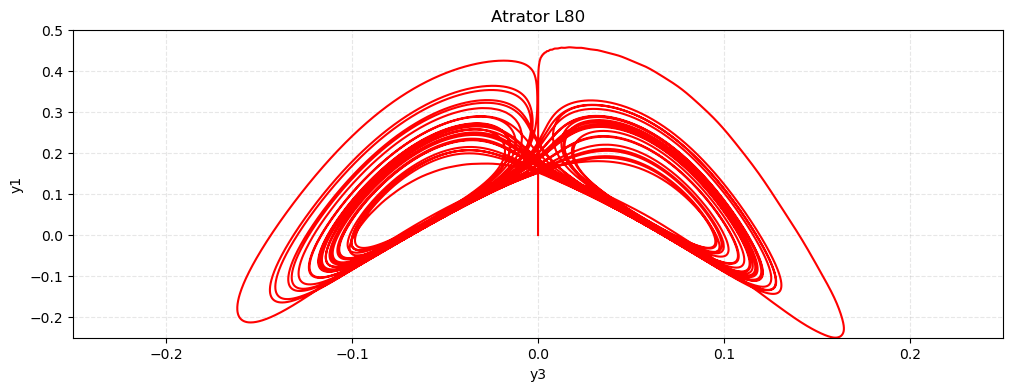
\includegraphics[width=0.7\textwidth]{img/p02y3y1.png}
		\caption{Hadley 01 - Projeção $y_3 \times y_1$}
		\label{fig:p02y3y1}
	\end{figure}
\end{frame}

%---------------------------------------------------

\begin{frame}{\textit{Modelo PE}: Resultados para condição de Hadley 01}
	\begin{figure}
		\centering
		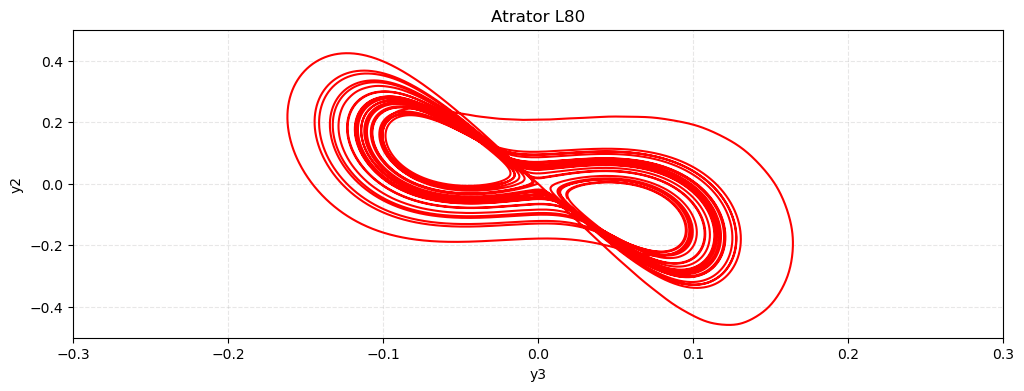
\includegraphics[width=0.7\textwidth]{img/p02y3y2.png}
		\caption{Hadley 01 - Projeção $y_3 \times y_2$}
		\label{fig:p02y3y2}
	\end{figure}
\end{frame}

%---------------------------------------------------

\begin{frame}{\textit{Modelo PE}: Resultados para condição de Hadley 01}
	\begin{figure}
		\centering
		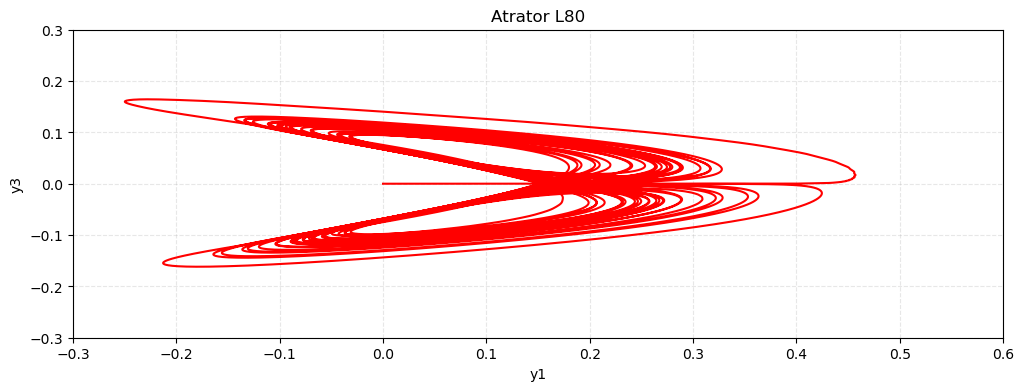
\includegraphics[width=0.7\textwidth]{img/p02y1y3.png}
		\caption{Hadley 01 - Projeção $y_1 \times y_3$}
		\label{fig:p02y1y3}
	\end{figure}
\end{frame}

%---------------------------------------------------

\begin{frame}[fragile]
	
	\frametitle{\textit{PE Model e QG Model}: Condições iniciais - Hadley 02}
	A presente condição reproduz as condições da circulação de Hadley de acordo com \cite{lorenz1980}
	\begin{python}
# Condições iniciais do modelo PE
x_hadley02_inicial = [-0.01111, 0, 0]
y_hadley02_inicial = [0.53331, 0, 0]
z_hardle02_inicial = [0.53354, 0, 0]
	\end{python}
	
	Equivalente a seguinte condição do QG Model:
	\begin{python}
# Condições iniciais do modelo QG
y0 = [0.53333, 0, 0]
	\end{python}
\end{frame}

%---------------------------------------------------

\begin{frame}{\textit{Modelo PE} e \textit{Modelo QG}: Resultados para a condição de Hadley 02}
	\begin{figure}
		\centering
		\begin{subfigure}[b]{0.45\textwidth}
			\centering
			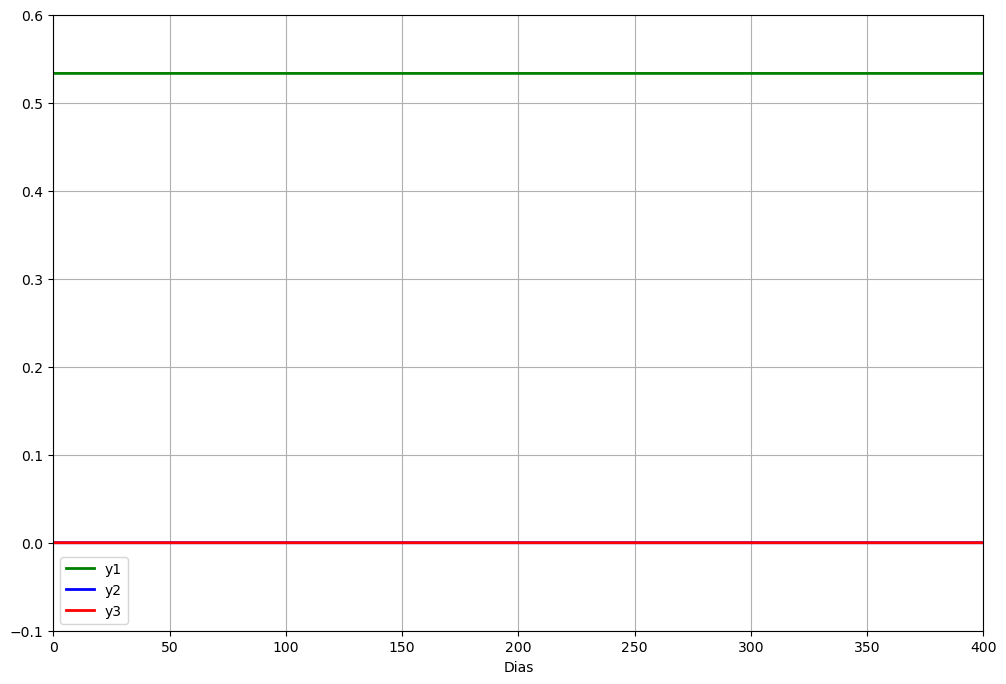
\includegraphics[width=\textwidth]{img/p03d400pe.png}
			\caption{Condição de Hadley 02 - 400 dias\\ (PE Model)}
			\label{fig:p03d400pe}
		\end{subfigure}
		\hfill
		\begin{subfigure}[b]{0.45\textwidth}
			\centering
			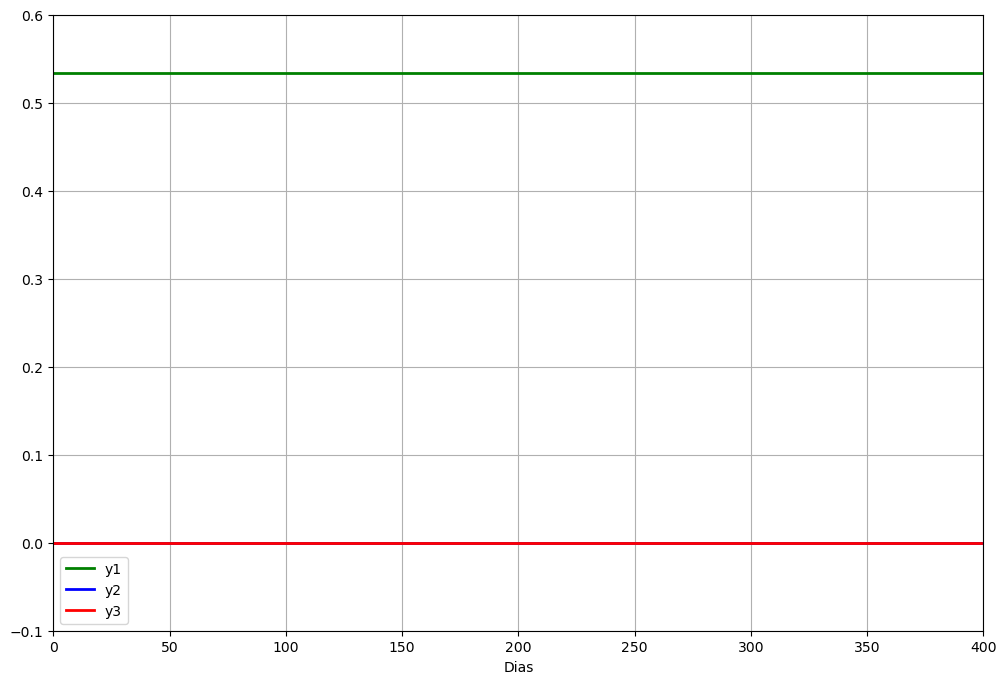
\includegraphics[width=\textwidth]{img/p03d400qg.png}
			\caption{Condição de Hadley 02 - 400 dias\\ (QG Model)}
			\label{fig:p03d400qg}
		\end{subfigure}
	\end{figure}
\end{frame}

%---------------------------------------------------

\begin{frame}{\textit{Algumas dificuldades}: As equações \eqref{eq:equacao-principal-simplificada-1}-\eqref{eq:equacao-principal-simplificada-3}}
	
	\begin{enumerate}
		\item Apesar das equações \eqref{eq:equacao-principal-simplificada-1}-\eqref{eq:equacao-principal-simplificada-3} serem simplificações de \eqref{eq:equacao-principal-1}-\eqref{eq:equacao-principal-3}, nenhuma das referências utilizadas utilizou as equações \eqref{eq:equacao-principal-simplificada-1}-\eqref{eq:equacao-principal-simplificada-3}
		\item Na tentativa de plotagem das \eqref{eq:equacao-principal-simplificada-1}-\eqref{eq:equacao-principal-simplificada-3}, houve diversos problemas, os principais foram: \textit{overflow} e desvio em relação a natureza das equações \eqref{eq:equacao-principal-1}-\eqref{eq:equacao-principal-3}
	\end{enumerate}
\end{frame}

%---------------------------------------------------

\begin{frame}{\textit{Algumas dificuldades}: As equações \eqref{eq:equacao-principal-simplificada-1}-\eqref{eq:equacao-principal-simplificada-3}}
		\begin{figure}
		\centering
		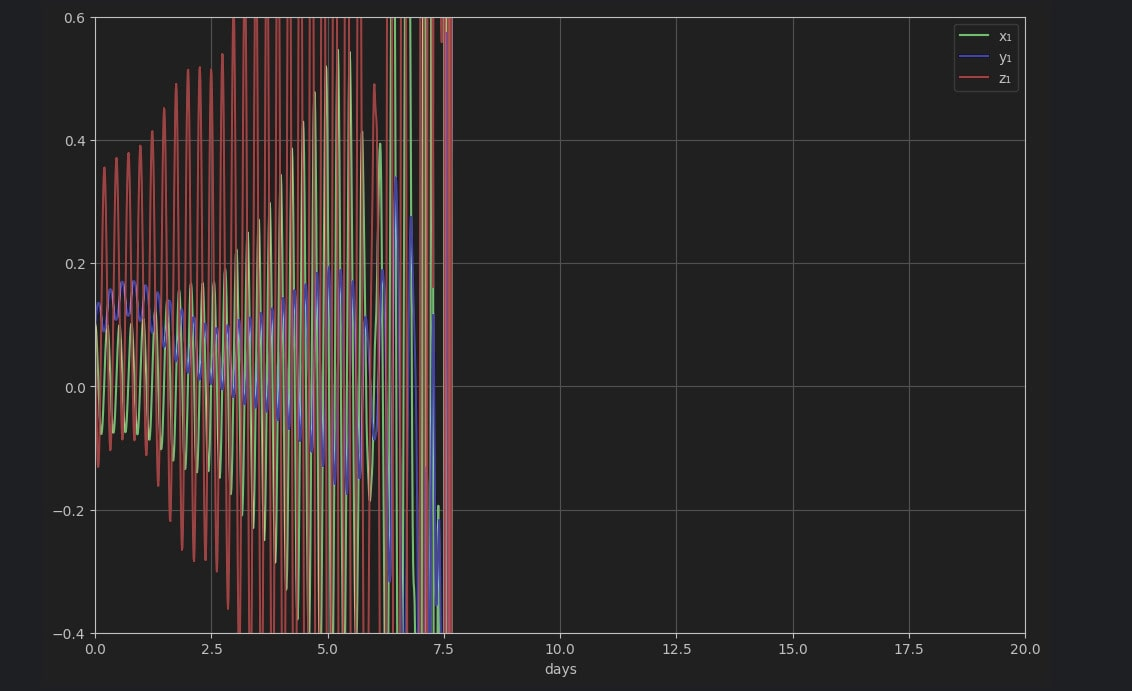
\includegraphics[width=0.5\textwidth]{img/erro_simplificado.jpeg}
		\caption{Tentativa de plotagem equações \eqref{eq:equacao-principal-simplificada-1}-\eqref{eq:equacao-principal-simplificada-3}}
		\label{fig:erro-plotagem-eq-simp}
	\end{figure}
\end{frame}

%---------------------------------------------------

\begin{frame}{\textit{Algumas dificuldades}: equações \eqref{eq:equacao-principal-1}-\eqref{eq:equacao-principal-3}}
	\begin{figure}
		\centering
		\begin{subfigure}[b]{0.45\textwidth}
			\centering
			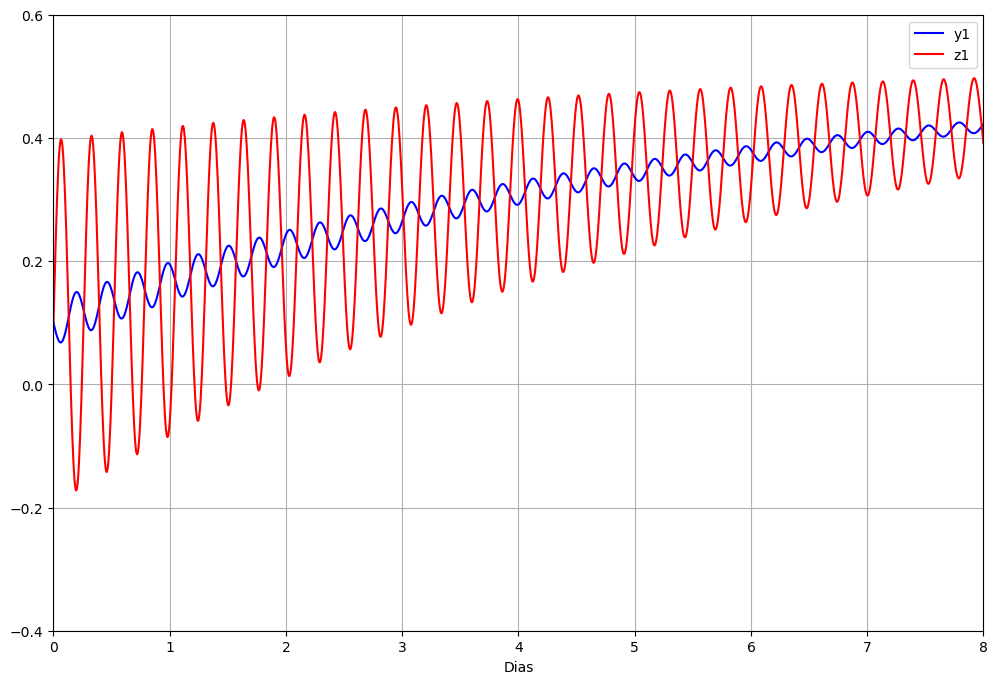
\includegraphics[width=\textwidth]{img/p01d08.png}
			\caption{Condição padrão - 8 dias}
			\label{fig:p01d08}
		\end{subfigure}
		\hfill
		\begin{subfigure}[b]{0.45\textwidth}
			\centering
			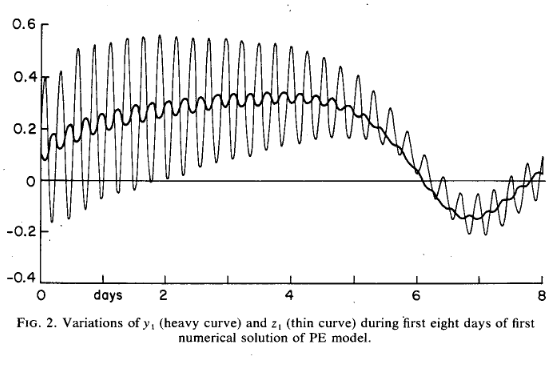
\includegraphics[width=\textwidth]{img/p01d08rel.png}
			\caption{Condição padrão - 8 dias (artigo)}
			\label{fig:p01d08rel}
		\end{subfigure}
	\end{figure}
\end{frame}
\section{Conclusão}

\begin{frame}{Repositório do Github}
\begin{center}
        \href{https://github.com/lucasamtaylor01/Lorenz80/blob/master/01_src/simulacoes.ipynb}{
        
\includegraphics[width=0.6\textwidth]{github.png}}
\end{center}

\end{frame}
\begin{frame}[allowframebreaks]{Referências}
    \nocite{*}
    \printbibliography[heading=none]
\end{frame}
\include{sections/section05}

% Slide final
\begin{frame}
    \begin{center}
        {\Huge Obrigado pela atenção!}
    \end{center}
\end{frame}

\end{document}


